\documentclass{standalone}
\usepackage[utf8]{inputenc}
\usepackage{siunitx}
\usepackage{tikz}
\usepackage{mathrsfs}
\usetikzlibrary{positioning, shapes.geometric, arrows}
\tikzstyle{startstop} = [draw, rectangle, rounded corners, minimum width=3cm, minimum height=1cm,text centered, draw=black]
\tikzstyle{bola} = [draw, circle , minimum size = 10, draw=black, text centered]
\tikzstyle{elipse} = [draw, ellipse, minimum height = 10]
\usepackage[T1]{fontenc}
\renewcommand*\familydefault{\ttdefault} %% Only if the base font of the document is to be typewriter style
\begin{document}
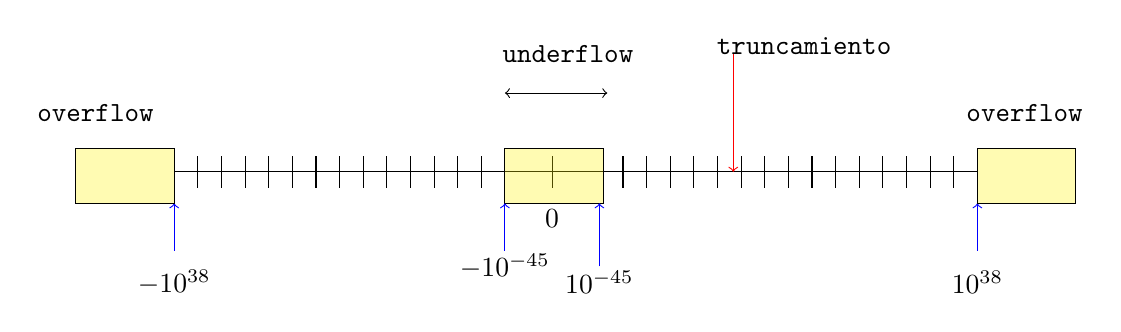
\begin{tikzpicture}
\draw (0, 3) -- (10.2, 3);
\draw (0, 3) -- (0, 2.7);
%\foreach \i in {3.2, 2.8}
\foreach \j in {0, 0.3, 0.6, ..., 4.2}
	\draw (\j, 2.8) -- (\j, 3.2);

\foreach \j in {5.7, 6.0, ..., 10.4}
	\draw (\j, 2.8) -- (\j , 3.2);

\draw (4.8, 3.2) -- (4.8, 2.8);

\draw [draw = black, fill = yellow, fill opacity = 0.3] (4.2, 2.6) rectangle ++(1.25, 0.7);
\draw (5, 4.5) node {underflow};
\draw [<->] (4.2, 4) -- (5.5, 4);

\draw (4.8, 2.4) node {$0$};
\draw (4.2, 1.8) node {$-\num{e-45}$};
\draw (5.4, 1.6) node {$\num{e-45}$};
\draw [->, color = blue] (4.2, 2.0) -- (4.2, 2.6);
\draw [->, color = blue] (5.4, 1.8) -- (5.4, 2.6);
\draw (0, 1.6) node {$\num{-e+38}$};
\draw [->, color = blue] (0, 2.0) -- (0, 2.6);
\draw (10.2, 1.6) node {$\num{+e+38}$};
\draw [->, color = blue] (10.2, 2.0) -- (10.2, 2.6);
\draw [draw = black, fill = yellow, fill opacity = 0.3] (-1.25, 2.6) rectangle ++(1.25, 0.7);
\draw (-1., 3.75) node {overflow};
\draw [draw = black, fill = yellow, fill opacity = 0.3] (10.2, 2.6) rectangle ++(1.25, 0.7);
\draw (10.8, 3.75) node {overflow};

\draw [->, color = red] (7.1, 4.5) -- (7.1, 3);
\draw (8, 4.6) node {truncamiento};
\end{tikzpicture}
\end{document}